\section{Theoretische Grundlage}
\label{sec:Theorie}
Bei dem Lock-In-Verstärker handelt es sich um einen Verstärker mit einem eingebautem phasenempfindlichem Detektor. Der Lock-In-Verstärker wird hauptsächlich zur Messung stark verrauschter Signale verwendet. Um dies zu realisieren wird das Meßsignal mit einer Referenzfrequenz $\omega_\text{0}$ moduliert. Die folgende Abbildung zeigt den schematischen Aufbau des Lock-In-Verstärkers:
\begin{figure}[H]
	\centering
	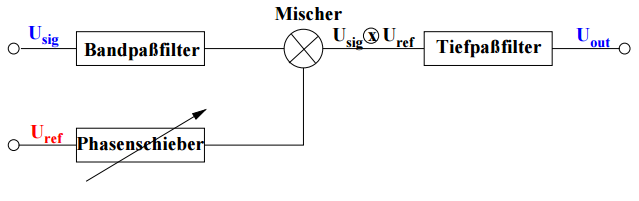
\includegraphics[height=4cm]{picture/sLIV.png}
	\caption{Schematischer Aufbau eines Lock-In-Verstärkers. \cite[1]{sample}}
  \label{img:sLIV}
\end{figure}
Das Nutzsignal $U_\text{sig}$ wird mit einem Bandpassfilter von Rauschanteilen höherer ($\omega \gg \omega_\text{0}$) und niedrigerer ($\omega \ll \omega_\text{0}$) Frequenzen gereinigt. Danach wird das Signal in dem Mischer mit einem Referenzsignal $U_\text{ref}$, welches die gleiche Frequenz wie $U_\text{sig}$ besitzt, multipliziert. Das Referenzsignal kann relativ zu dem Nutzsignal Phasenverschoben werden und so mit dem Signal synchronisiert werden ($\Delta \Phi = 0$). Der nachfolgende Tiefpaß ($\tau = RC \gg 1/ \omega_\text{0}$) integriert das Mischsignal $U_\text{sig} \times U_\text{ref}$
über mehrere Perioden der Frequenz $\omega_\text{0}$. Dadurch wird eine großer Teil der Rauschbeiträge, welche nicht mit der Frequenz des Nutzsignals synchronisiert sind, herausgemittelt. Durch dieses Verfahren wird am Ausgang eine zur Eingangsspannung $U_\text{sig}$ proportionale Gleichspannung $U_\text{out} \propto U_\text{0} \cdot \cos \Phi$ gemessen. Außerdem definiert dieser Tiefpass auch die Bandbreite des Restrauschens, wenn die Zeitkonstante $\tau = RC$ sehr groß gewählt wird, wird die Bandbreite $\Delta \nu = 1/(\pi RC)$ belibieg klein. So wird mit dem Lock-In-Verstärker ein Güte von $Q = 100000$ erreicht, währenddessen kann ein Bandpass nur Güten von $Q = 1000$ erreichen.
\begin{figure}[H]
	\centering
	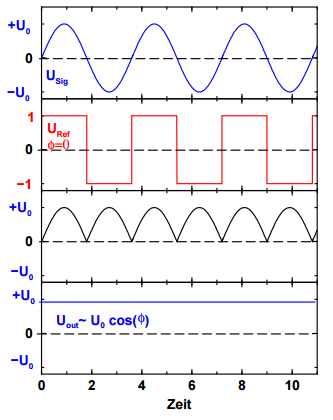
\includegraphics[height=8cm]{picture/SV.png}
	\caption{Signalverläufe. \cite[2]{sample}}
  \label{img:SV}
\end{figure}
In Abblidung \ref{img:SV} wird eine sinusförmige Signalspannung
\begin{align}
	U_\text{sig} = U_\text{0} \sin(\omega t) \ ,
\end{align}
betrachtet, die durch $U_\text{ref}$ moduliert wird. $U_\text{ref}$ hat dabei eine auf 1 normierte Amplitude, die bei einer positiven Signalspannung auf 1 steht und bei einer negativen Signalspannung auf -1 steht. Dadurch wird das Nutzsignal von einer Wechselspannung zu einer Gleichspannung geändert, um bei der Integration ein Ergebniss ungleich 0 zu erhalten. %ist der letzte satz notwendig?
Die Rechteckspannung $U_\text{ref}$ wird mit einer Fourrierreihe genähert, die sich aus den ungeraden Harmonischen der Grundfrequnz $\omega$ zusammensetzt und die Form
\begin{equation}
	U_\text{ref} = \frac{4}{\pi} \left( \sin(\omega t) + \frac{1}{3} \sin(3 \omega t) + \frac{1}{5} \sin(5 \omega t) + ... \right)
\end{equation}
hat. Nach dem multiplizieren von der Signalspannung mit der Rechteckspannung folgt, dass
\begin{equation}
	U_\text{sig} \times U_\text{ref} = \frac{2}{\pi} \left(1 - \frac{2}{3} \cos(2 \omega t) - \frac{2}{15} \cos(4 \omega t) - \frac{2}{35} \cos(6 \omega t) - ... \right)
	\label{eqn:foye}
\end{equation}
ist. Das entspricht nun der geraden Oberwelle der Grundfrequenz $\omega_\text{0}$. Danach durchläuft die gerade Oberwelle den Tiefpassfilter und wird zu einer Gleichspannung, die proportional zur Signalspannung ist,
\begin{equation}
	U_\text{out} = \frac{2}{\pi} U_\text{0} \ .
	\label{eqn:Uout1}
\end{equation}
Wenn die Signalspannung und die Referenzspannung nicht in Phase sind folgt mit Abbildung \ref{img:SV} und Gleichung \ref{eqn:Uout1}:
\begin{equation}
	U_\text{out} = \frac{2}{\pi} U_\text{0} \cos(\Phi) \ .
	\label{eqn:Uout2}
\end{equation}
\newpage

\subsection{Fehlerrechnung}
Sämtliche Fehlerrechnungen werden mit Hilfe von Python 3.4.3 durchgeführt.
\subsubsection{Mittelwert}
Der Mittelwert einer Messreihe $x_\text{1}, ... ,x_\text{n}$ lässt sich durch die Formel
\begin{equation}
	\overline{x} = \frac{1}{N} \sum_{\text{k}=1}^\text{N} x_\text{k}
	\label{eqn:ave}
\end{equation}
berechnen. Die Standardabweichung des Mittelwertes beträgt
\begin{equation}
	\Delta \overline{x} = \sqrt{ \frac{1}{N(N-1)} \sum_{\text{k}=1}^\text{N} (x_\text{k} - \overline{x})^2}
	\label{eqn:std}
\end{equation}

\subsubsection{Gauß'sche Fehlerfortpflanzung}
Wenn $x_\text{1}, ..., x_\text{n}$ fehlerbehaftete Messgrößen im weiteren Verlauf benutzt werden, wird der neue Fehler $\Delta f$ mit Hilfe der Gaußschen Fehlerfortpflanzung angegeben.
\begin{equation}
	\Delta f = \sqrt{\sum_{\text{k}=1}^\text{N} \left( \frac{ \partial f}{\partial x_\text{k}} \right) ^2 \cdot (\Delta x_\text{k})^2}
	\label{eqn:var}
\end{equation}

\subsubsection{Lineare Regression}
Die Steigung und y-Achsenabschnitt einer Ausgleichsgeraden werden gegebenfalls mittels Linearen Regression berechnet.
\begin{equation}
	y = m \cdot x + b
	\label{eqn:reg}
\end{equation}
\begin{equation}
	m = \frac{ \overline{xy} - \overline{x} \overline{y} } {\overline{x^2} - \overline{x}^2}
	\label{eqn:reg_m}
\end{equation}
\begin{equation}
	b = \frac{ \overline{x^2}\overline{y} - \overline{x} \, \overline{xy}} { \overline{x^2} - \overline{x}^2}
	\label{eqn:reg_b}
\end{equation}
\newpage
